\documentclass[10pt,a4paper,twocolumn]{article}
\usepackage[utf8]{inputenc}
\usepackage[T1]{fontenc}
%\usepackage{gentium}
\usepackage{mathptmx} % Use Times Font
\usepackage{amsmath}
\usepackage{graphicx} % Required for including pictures
\usepackage{hyperref} % Format links for pdf
\usepackage{biblatex}
\addbibresource{references.bib}
\usepackage{booktabs} % Used so that tables generated by pandas
                      % to_latex() work correctly

\frenchspacing % No double spacing between sentences
\usepackage[margin=1in]{geometry}

\usepackage[all]{nowidow} % Tries to remove widows
\usepackage[protrusion=true,expansion=true]{microtype} % Improves typography, load after fontpackage is selected

\usepackage{lipsum} % Used for inserting dummy 'Lorem ipsum' text into the template

\title{descriptive title about chess}
\author{Leon Lee and Lila Marshman}

\begin{document}

\maketitle

%% INSTRUCTIONS:
%%
%% 1. Create your own copy of this Overleaf project. You can either edit your report
%% using:
%%
%%    a. Overleaf professional, a collaborative LaTeX editor. You can click
%%       "Copy Project" from the Overleaf menu to create a version where you have
%%       read and write permissions. See the following for documentation:
%%       https://www.overleaf.com/edu/edinburgh and
%%       https://uoe.sharepoint.com/:f:/r/sites/digitalskillsandtraining/Shared%20Documents/LaTeX/LaTeX%20for%20Beginners%20using%20Overleaf?csf=1&web=1&e=cPqTI3
%%
%%    b. A LaTeX editor on your PC. For this option, you can download the source
%%       of this project as a zip (via the Overleaf menu).
%% 
%% 2. Please rename this file fds-project-option-1.tex, 
%% fds-project-option-2.tex, or fds-project-option-3.tex, depending on
%% which project option you are doing. When you submit, please submit
%% the PDF file with the corresponding name.
%% 
%% 3. Please keep the section and paragraph headings as they
%%    are. You should delete all the text within the headings, e.g.
%%    the text that says "What is the area of this data science
%%    study, and why is it interesting to investigate" and the
%%    bullet points. Keeping the headings makes the report a lot
%%    easier for the markers to read, and making things easy for
%%    markers is always beneficial.
%%
%% 4. The word limit for the Overview section is mandatory. For the
%% other sections word limits are suggested.
%%
%% 5. The page limits must be strictly adhered to, and depend on if
%% you are working individually, in pairs or in threes:
%%
%%   - Individual: 6 pages 
%%   - Pairs: 8 pages 
%%   - Threes: 10 pages 
%%

\section{Overview}
% 250 words maximum


Online chess sites receive a huge amount of game data from large volumes of users accessing and playing on their sites. Many have large player bases, representing a huge variety in player ELO scores (a number corresponding to skill level). We used data from Chess.com to analyse the relevancy of players' ELO in a chess game. A logistic regression model was used to investigate the effect of the difference in ELO on winning a game. We proposed an exponential function 'Temptation' to be used as a hyperparameter for a predictive model. This model investigated the possibility of predicting ELO from the context of particular game states. We chose to specifically investigate the game states where an 'en passant' move was performed. [Lila Talk about evaluation and results]

Visualisations of ...
Statistical techniques used ...

\section{Introduction}
% Suggested 400 words

\paragraph{Context and motivation}

Online chess sites such as Chess.com allow users may play with friends or strangers, offering a wide variety of chess variants and time controls to play with. Its rise in popularity follows the increase in free time during the COVID-19 pandemic lockdowns, the popularity of Netflix's show 'The Queen's Gambit', and world-ranking players streaming the game on Twitch \cite{The2020ChessBoom} With a sudden increase in online players comes an increase in publicly available game data. This provides the opportunity for an investigation into player's strengths, measured by ELO.

[Lila where? to put this bit:]

This report studies a dataset of 60,000 games, analysing the impact a difference in ELO (score related to playing ability in chess) makes on the outcome of a game. We also consider whether ELO may be predicted from a player's response to an 'en passant' move.

\paragraph{Previous work}

Brief description of any previous work in this area (e.g., in the
media, or scientific literature or blogs).

An article in the literature found [Lila put what it found] about the ELO \cite{HowMuchDoesEloMatter}.
There is no literature directly studying the relationship between a player's response to 'en passant' moves and their ELO.
\paragraph{Objectives}

% What questions are you setting out to answer?
Commonly, chess tactics are a way to gain an inherent advantage in the game state. Thus, a highly ranked chess player could plan ahead several moves just to obtain this state. Common tactics are ones that most players that are somewhat into chess will recognise as an advantageous move, but being able to consistently plan to apply the knowledge is what separates a good chess player from a great one. However, one exception to this is the move \textit{en-passant}. This is a far more situational tactic, and heavily relies on your opponent to move a certain way for a player to be able to utilise it. More importantly, often it does not leave the board in an advantageous state for the moving player. Due to this, compared to most other chess tactics, generally using en-passant will not be the optimal move. Therefore, if you are highly ranked and playing to win, chances are that you would not take it given the chance. However, in the chess scene, and especially in online chess which is where this dataset is sourced from, the move has gained a cult-like following. Since most people that are active in the online chess scene will be lower elo, we can use this fact to try and predict the elo of an individual player based on the chance they will take an en-passant, since we can assume that the higher the elo you are, the less likely to take it

\section{Data}
% Suggested 300 words

% Who created the dataset(s)?  How you have
% obtained it (e.g., file or web scraping), and do the T\&Cs allow you
% to use obtain the data for the project?

\paragraph{Data provenance}
We obtained our data from Kaggle.com \cite{Kaggle}, where they provided a dataset of over 60,000 games of chess taken from Chess.com. The User Agreement on Chess.com states that you are not allowed to data mine \cite{ChessT&C}, but in this case the dataset was extracted using the Chess.com API so it complies with their regulations.

% Description of the data, e.g. variables
% in each table, number of records.
\paragraph{Data description}
The dataset records $66,879$ games of chess that took place on Chess.com with varying game modes, time classes, and levels of players. The data is all in one file but the columns are effectively split up into two sections. The first are the main columns, while the final column is the PGN. The main columns include basic data i.e. the usernames and links of players, the ELO ratings of each player, the result of both players, the time control and time class, the rules the game was played on, and the final board state. On the other hand, the PGN (Portable Game Notation) is a column in a standard format to be easily read by other chess analysers. Thus it has a lot of the same information the previous fields do, but it also includes important information like the opening moves, and especially the last field which is a list of all the moves that took place during that game. Using the PGN we can simulate and replay exactly how the game was played, and analyse using that.

% How you have processed the dataset, e.g.,
% cleaning, removing missing values, joining tables.
\paragraph{Data processing}
The data was well set out, so it did not need much cleaning in terms of removing invalid entries or NaN values. However, since the dataset includes lots of different modes of games, some which are not standard chess, we removed them since they wouldn't be an accurate representation of an average chess game. One example of a chess variation is Chess960, where the starting positions of the pieces are randomised.
We also removed games where the game terminated early - either from timeout, resignation or other means. We used two filters, the first being to read the top row of the end-board, and if the pieces are laid out in the order "RNBKQBNR", that's an indicator that the game has not developed much since all the important pieces are in their starting place. Our second method was to filter out any games with less than 10 total moves (or 5 per player). We concluded that any games in these two categories would not be useful to the data analysis.

\section{Exploration and  analysis}
% Suggested 500 words for individual report; proportionately longer
% for group projects).

% 't' means "try to position at the top of the page"
\begin{figure*}[t]
  \centering
  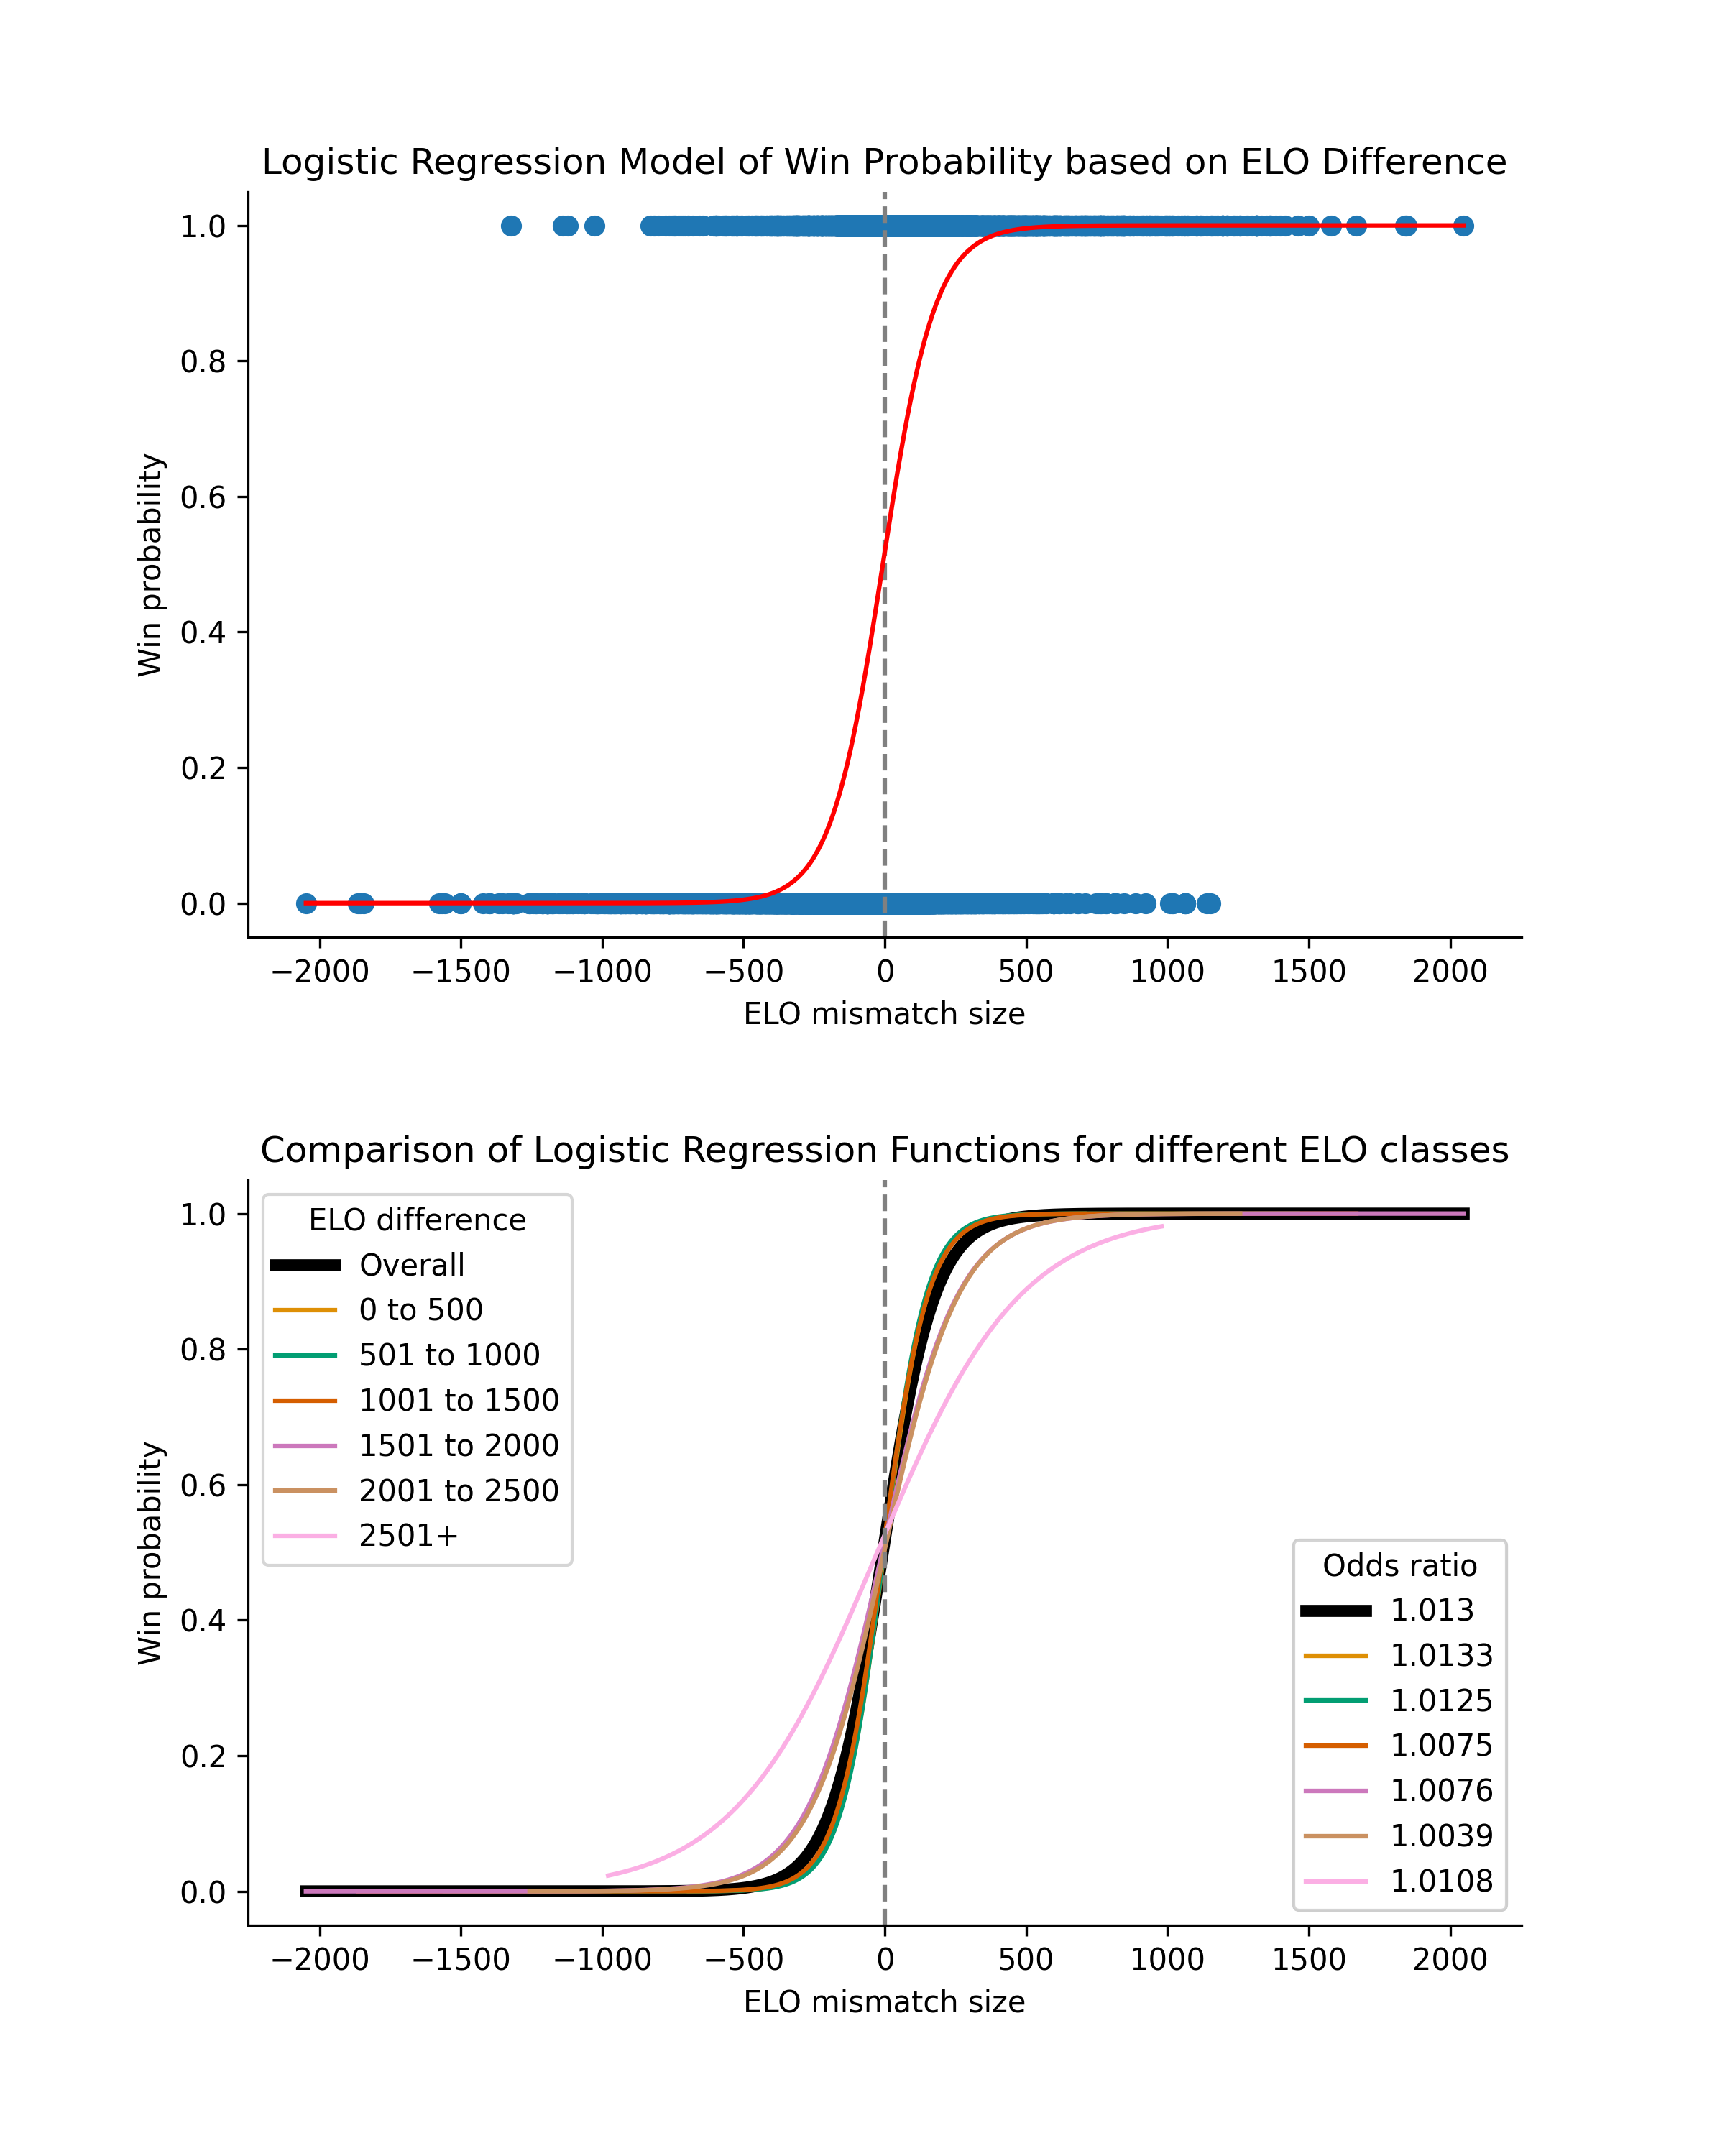
\includegraphics{report/images/log_regression_dual.png}
  \caption{Each datapoint represents how many ELO points a player is than their opponent during a game, and whether they won (1) or lost (0). The standard logistic function is plotted in red.
  Demonstration figure. This caption explains more about the figure. Note that the font size of the labels in the plot is 9pt, which is obtained by the settings as shown in the Jupyter notebook.}
  \label{fds-project-template:fig:log_regression}
\end{figure*}

% 'b' means "try to position at the bottom of the page"

\paragraph{Data Analysis: Question 1}
To investigate the association between the difference in players' ELO and winning, we used a logistic regression model. We believed this to be the most appropriate model to use since it works well for data with a continuous predictor (ELO difference) and a binary response variable (winning or losing). To ensure a binary outcome, we excluded games which ended in a draw or other indeterminate end-states.
One of the dataset columns was 'time class' which classified games into $4$ categories depending on their maximum allowed length: 'daily', 'rapid', 'blitz' and 'bullet'. However, the dataset contained relatively few 'daily' games which, if we randomly sampled the dataset, may have led to these 'daily' games holding a larger weight, thus not accurately representing the total population of all games in the dataset.
To reduce these effects we took a stratified sample, proportionally sampling by 'time class'. This resulted in a sample size of $n={something}$, with ELOs ranging from ${something around -2k}$ to ${something around 2k}$. \newline

We then split the sample into a training set and test set at an $80:20$ ratio so that we could evaluate the model's performance. This was because we wanted to see how accurately it represented an association between the two investigation variables [Lila check this].

After applying the logistic regression to the training set of data we found $\beta_{0}$ and $\beta_{1}$ to be $0.0768$ and $0.0103$ respectively. We used $\beta_{0}$ to calculate the probability of a win for players of the same ELO as 
$$\displaystyle\frac{1}{1+e^{\beta_{0}}} = 0.48081$$
This is close to the intuitively expected value of $0.5$, where a win or a loss is equally likely. Since the log odds, $\beta_{0}$, for players with the same ELO is close to $0$ ($0.0768$ logits), then winning and losing are almost equally likely in this case. Furthermore, the odds ratio, $e^{\beta_{0}} = 1.0103$ shows that for every 1 point higher a player is in ELO, they are $1.0103$ times more likely to win. \newline

The logistic regression model was estimated using maximum likelihood, so it seemed most appropriate to use a Wald test to test for a relationship between ELO difference and the probability of a win \cite{WaldTest}. We used the null hypothesis $H_{0}: \beta_{1} = 0$ which states there is no statistically significant relationship, and alternative hypothesis $H_{a}: \beta_{1} \neq 0$ which suggests there is a statistically significant relationship. Following the test procedure outlined by Forthofer, Lee and Hernandez \cite{WaldTest}, and a method to calculate the Wald statistic inspired by StackExchange user j\_sack \cite{StackExchangeWaldTest}, we found a Wald statistic of $75.3946$, which gave a p-value of $p<0.01$. Thus we may reject the null hypothesis at the $1\%$ level, concluding there is insufficient evidence to support there not being a statistically significant relationship between ELO difference and probability of winning. \newline

Furthermore, when applying the model to the test set and comparing its predictions with the actual outcomes, we found an AUC score of $0.6987$. This implies a decent performance of the model, sugesting the logistic regression model can relatively accurately predict an outcome when given an ELO difference. This would not have been the case if there was no association between these variables. \newline




\paragraph{Data Analysis: Question 2 - Using a model based on temptation of en-passant to predict ELO}
To find a suitable model to predict ELO based on the context of an en-passant move, we utilised various external libraries to assist our data exploration. Using the \textit{python-chess} library [TODO: cite?], we were able to parse the "pgn" field to obtain information for each game in the dataset. Using these tools, we were first able to filter out the games that included an en-passant opportunity ($n=5074$), along with the games where an en-passant move actually occurred ($n=1563$). We then used \textit{Stockfish}[TODO: cite?], an open source chess game engine, to evaluate how well certain moves perform. Using the board state right before an en-passant opportunity, we were able to obtain how much of an advantage a player would gain from the following moves: a Stockfish calculated best move, the move the player decided to play, and finally the relevant en-passant capture (if both sides have opportunity, then the higher evaluated move is chosen).\newline

From these evaluations, we were able to use our results to create a model to predict human behaviour of an en-passant capture. If we assume the best move of a certain board state is the upper limit of a persons choice, then we can think of the likelihood of picking any other move as a function that grows exponentially small [LILA see if can find something to prove its exponential] by some factor depending on the evaluation difference, since the likelihood of picking a move that puts you in an advantage $T(move)$ (close to the best move), would be a lot more viable than picking a move that puts you in a large disadvantage (far from the best move). We will call this the temptation of a move, and is modelled like so:
$$T(\text{move})= -e^{(E_{\text{best}} - E_{\text{move}})/{n}} + 1$$
where $n$ is some factor to stop the exponential function from growing too quick. We tested on various different factors, but we didn't find any clear patterns so we settled on $n=220$. This value of $n$ gave the highest peak of $65\%$ accuracy across $1,000$ tests, and an average accuracy of $63\%$ across $10,000$ tests. The highest temptation is $0$ i.e. when the best move is the same as the specified move, in this case it would be if the best case was also en-passant. Using more variables such as the current board's evaluation, you could obtain a more accurate and in-depth, model but this one works for our case. \newline

After calculating the temptation of every en-passant move, we found the probability that someone in a certain ELO would play an en-passant move. There isn't enough samples in the dataset to get any meaningful information from comparing single values, since there is a large range of $2000+$ ELOs and only around $5000$ entries, so we rounded each player's ELO to the nearest $10$ and calculated the probability using that. Once we had probabilities for every player, we plotted temptation against the percent probability of playing an en-passant move. Players are split up into three different categories, which are a general grouping of low, average, and high elo players. The ELO splits are taken from the distribution of average ELO across players in the dataset ($\mu=1240.6,\,\sigma^{2}=399.3$), where the average ELO is $\pm 1\text{SD}$, and the low/high ELO splits are any values to the left and right of that section respectively. (Fig. \ref{fds-project-template:fig:temptation}).\newline

From the chart, we can see that higher ELO players have a much higher probability of playing en-passant; high ELO players are the only ones with above 60\% play rate in some cases.  But, for the most part they will only consider when the temptation is high. On the other hand, average ELO players are not as certain in terms of probability, but they do consider en-passant as a much more viable move even if it puts them in a considerable disadvantage. Low ELO players are similar to average ELO players, but slightly lower. This is excpected, as some lower ELO players might not know how or when to actually play en-passant. \newline

We then analysed the dataset using PCA to reduce the dimensionality, and then split the data into a training and testing set in an 60:40 ratio respectively. We used this ratio because any wider a difference and the model would overfit/underfit the data [Lila work out which one it is] meaning the confusion matrix wouldn't [Lila finish this]. We modelled a k-nearest neighbours estimator on the training set to predict the ELO class of a player, which is visualised in a chart (Fig. \ref{fds-project-template:fig:knn}). From the k-nearest neighbours chart, the left and right sides are relatively well defined, but the middle has a wider spread of data, which would likely result in a large error rate: there are points from all three categories overlapping, making it difficult to accurately predict the class a data point inside that region would end up in. \newline

We created a confusion matrix (displayed as a table in Fig [Lila cite]) detailing the numbers of correct and incorrect predictions of the k-NN model on the test set for each ELO class. Here we see $ LILA $ out of $LILA$ were predicted correctly for the high ELO class, $LILA$ out of $LILA$ for the medium ELO class and $0$ out of $LILA$ for the low ELO class. Values from the confusion matrix were used to calculate metrics to evaluate the model's predictive performance. These metrics were: accuracy ($0.65$), precision ($0.8463$), recall ($0.6270$), and sample-weighted F1 score ($0.7168$). The accuracy is reasonably above $0.5$, thus demonstrating slight success in our model's predictive capabilities, with room for refining the model. The precision score and recall score were used in the calculation for the F1 score, which evaluates the model for precision (amount of correctly classified data points) and robustness (whether it misses a significant amount of data) \cite{MetricsToEvaluateYourML}. To account for the test set containing different proportions of each ELO class, we used the sample-weighted calculation for the F1 score. This produced an F1 score of $0.7168$ which shows an okay fit of the model to the data, with room for improvement. \newline

We further produced an ROC [Lila do this and cite figure]

\begin{table*}[b]
  \centering
  \caption{Excerpt from Scottish Index of Multiple Deprivation, 2016 edition.
    \url{https://simd.scot}. You may put more information in the caption.}
  \label{tab:example1}
\begin{tabular}{lrrrrrrr}
\hline\hline
\textbf{Location}&\textbf{Employ-}&\textbf{Illness}&\textbf{Attain-}&\textbf{Drive}  &\textbf{Drive}    &\textbf{Crime}&\dots\\
                 &\textbf{ment}   &                &\textbf{ment}   &\textbf{Primary}&\textbf{Secondary}&              &\\
\hline
\textbf{Macduff}&$10$&$ 95$&$5.3$&$1.5$&$6.6$&$249$&\dots\tabularnewline
\textbf{Kemnay}&$ 3$&$ 40$&$5.3$&$2.4$&$2.4$&$168$&\dots\tabularnewline
\textbf{Hilton}&$ 0$&$ 10$&$6.3$&$2.2$&$3.0$&$144$&\dots\tabularnewline
\textbf{Ruchill}&$ 8$&$130$&$4.9$&$1.7$&$5.6$&$318$&\dots\tabularnewline
\textbf{Belmont}&$ 2$&$ 50$&$6.1$&$3.1$&$3.2$&$129$&\dots\tabularnewline
\dots&\dots&\dots&\dots&\dots&\dots&\dots&\dots\tabularnewline
\hline
\end{tabular}
\end{table*}


\begin{figure}[t]
  \centering
  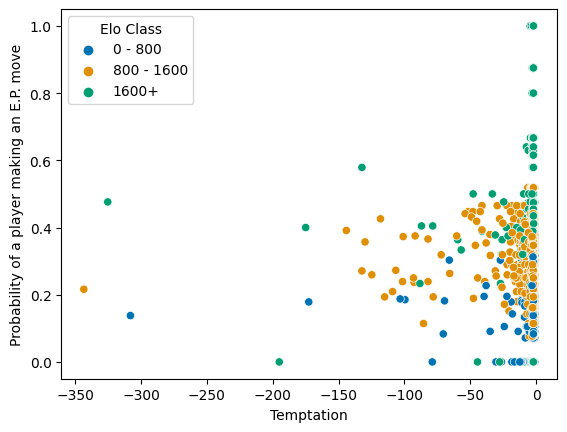
\includegraphics{report/images/temptation_chart.png}
  \caption{descriptive caption that i cba doing rn}
  \label{fds-project-template:fig:temptation}
\end{figure}

\begin{figure}[t]
  \centering
  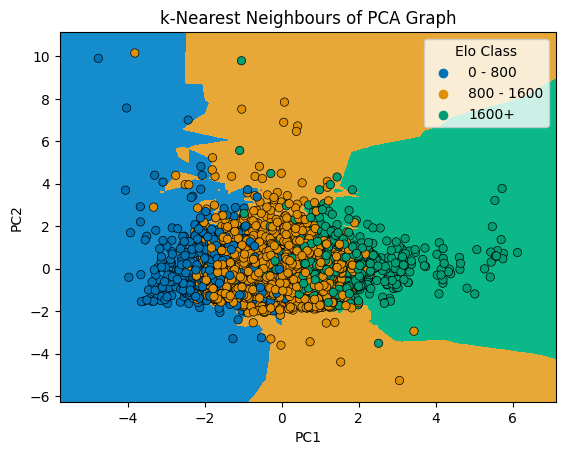
\includegraphics{report/images/knn_graph.png}
  \caption{another descriptive caption that i cba doing rn}
  \label{fds-project-template:fig:knn}
\end{figure}

\begin{figure*}[t]
  \centering
  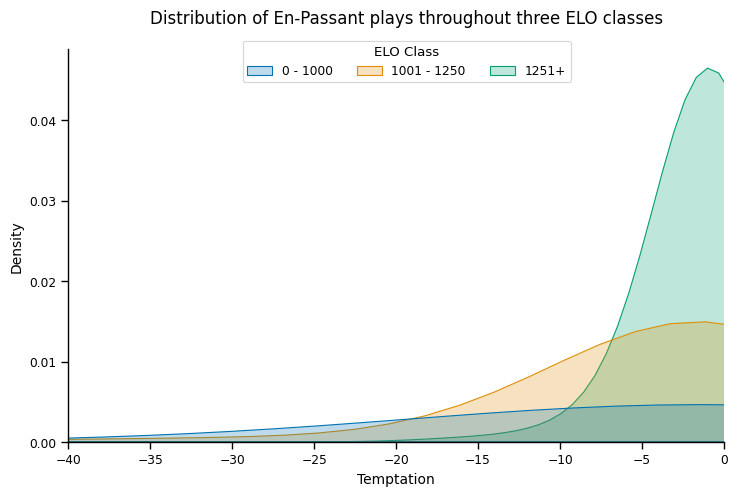
\includegraphics{report/images/ep_distplot.png}
  \caption{another descriptive caption that i cba doing rn}
  \label{fds-project-template:fig:knn}
\end{figure*}

% From k-NN we were unable to find a suitable model to predict ELO based on en passant context. We conducted a K-Means partitional clustering method on the data to further demonstrate that it is unlikely to find a suitable model using specifically these hyperparameters. If after conducting this we find no similar clusters of data at all, then it would be expected that we cannot group data by these hyperparameters, thus we cannot predict ELO from these.

% To find the best number of clusters $k$, we used the elbow method on a scree plot. The scree plot [Lila cite the figure] plotted the standard squared error (SSE) for data point variations in their clusters [Lila double check that's what this is] for values $1 < k <= 25$ suggests points near $k = 8$ are potential 'elbow' point candidates. We chose $k = 8$ as our number of clusters.
% We applied PCA to reduce the dimensionality of 5 hyperparameters before applying the K-Means. Standardised to ensure all variables had the same scale, so K-Means wouldn't be affected by [LILA SEE P11 FAILURE OF K MEANS SECTION IN LECTURE NOTES] The graph of the K-Means shows 8 different clusters, differentiated by colour-vision-deficiency-friendly colours, with the centres of each cluster marked by a black cross. With the exception of group $4$, all clusters overlap significantly. This implies the model is overfitted/underfitted[LILA work out which one and explain better].



\section{Discussion and conclusions}
% Suggested 400 words.

\paragraph{Summary of findings}

\paragraph{Evaluation of own work: strengths and limitations}

\paragraph{Comparison with any other related work}
E.g. ``Anscombe has also demonstrated that many patterns of data can
have the same correlation coefficient'' \cite{anscombe1973graphs}.

Wikipedia can also be cited but it is better if you find the original
reference it for a particular claim in the list of references on the
Wikipedia page, read it, and cite it.

The golden rule is always to cite information that has come from other
sources, to avoid plagiarism \cite{wiki:plagarism}. \cite{HowMuchDoesEloMatter}

\paragraph{Improvements and extensions}

\printbibliography
\end{document}

% LocalWords:  lrrrrrrr ment Macduff Kemnay Ruchill FDS mc th fds
% LocalWords:  Anscombe dataset